\phantomsection
%\addcontentsline{toc}{chapter}{Introduzione}
\chapter{Rappresentazione grafica delle Dipendenze Funzionali Rilassate}
\markboth{Rappresentazione grafica delle Dipendenze Funzionali Rilassate}{}
\label{cap4:visual_representation}
% [titolo ridotto se non ci dovesse stare] {titolo completo}

Data la possibilit\`{a} per le \acrshort{rfd} di utilizzare confronti approssimati e misure di copertura per specificare il sottoinsieme di tuple a cui appartengono, i loro algoritmi di ricerca spesso producono in output enormi insiemi di dipendenze, impedendo ad un utente di coglierne facilmente informazioni e statistiche. A tal fine, vengono proposte due strategie per affrontare questo problema in \cite{mdvisualization}: si filtrano le RFD pi\`{u} rilevanti tramite il concetto di minimalit\`{a} e le si rappresentano attraverso diverse metafore di visualizzazione, dove ognuna delle quali mette in risalto un aspetto differente.

\section{Minimalit\`{a} delle RFD}
Come detto in precedenza, la minimalit\`{a} \`{e} una propriet\`{a} che pu\`{o} essere sfruttata per concentrarsi su un insieme di \acrshort{rfds} significative, poich\'{e} consente di eliminare alcune \acrshort{rfds} valide che possono essere derivate da altre. Tale propriet\`{a} \`{e} stata gi\`{a} analizzata nel contesto delle \acrshort{fds}, dove si utilizza la regola di interferenza di Armstrong per derivare l'insieme minimale delle \acrshort{fds}. Pi\`{u} specificamente, un insieme di \acrshort{fds} pu\`{o} considerarsi minimale se e soltanto se contiene solamente:
\begin{enumerate}
    \item \acrshort{fds} non banali,
    \item \acrshort{fds} con il minor numero possibile di attributi sul lato sinistro,
    \item \acrshort{fds} che non possono essere derivate da altre attraverso la propriet\`{a} della transitivit\`{a}.
\end{enumerate}\par
Per estendere tale concetto nel contesto delle \acrshort{rfds}, \`{e} necessario introdurre dei parametri addizionali di minimalit\`{a}, come le funzioni di distanza o di somiglianza e le soglie associate. Ad esempio, supponiamo di avere le seguenti tre \acrshort{rfds} su un'istanza $r$ di una relazione $R=\{A,B,C\}$:
\begin{enumerate}
    \item $A_{\leq2},B_{\leq2}\rightarrow C_{\leq1}$,
    \item $A_{\leq2},B_{\leq1}\rightarrow C_{\leq3}$,
    \item $A_{\leq3}\rightarrow C_{\leq1}$.
\end{enumerate}
Sebbene le prime due abbiano gli stessi attributi sul lato destro e sul lato sinistro, le loro soglie di distanza sono differenti, mentre la terza ha la cardinalit\`{a} del lato sinistro diverso. Analizzando la seconda \acrshort{rfd}, questa afferma che ogni coppia di tuple che hanno una distanza minore o uguale a 2 sull'attributo $A$ e minore o uguale ad 1 sull'attributo $B$, allora hanno una distanza minore o uguale a 3 sull'attributo $C$. Dato ci\`{o}, la prima \acrshort{rfd} presenta un lato sinistro pi\`{u} generale (i.e., $B_{\leq2}$ include $B_{\leq1}$) ed un lato destro pi\`{u} restrittivo (i.e., $C_{\leq1}$ \`{e} incluso in $C_{\leq3}$), essendo pi\`{u} restrittiva su un insieme pi\`{u} grande di coppie di tuple candidate per il lato sinistro. Di conseguenza, la seconda \acrshort{rfd} non \`{e} minimale. Inoltre, la prima \acrshort{rfd} non \`{e} minimale rispetto la terza, dato che la terza \acrshort{rfd} non solo ha una soglia pi\`{u} alta sull'attributo $A$, ma contiene anche un numero minore di attributi sul lato sinistro.\par
Pi\`{u} specificamente, un insieme di \acrshort{rfd} si dice minimale se e soltanto se questo contiene:
\begin{enumerate}
    \item \acrshort{rfds} non banali,
    \item \acrshort{rfds} con il minor numero possibile di attributi sul lato sinistro,
    \item \acrshort{rfds} con le soglie massime possibili per gli attributi sul lato sinistro,
    \item \acrshort{rfds} con le soglie minime possibili per l'attributo sul lato destro.
\end{enumerate}

\section{Rappresentazione visuale delle RFD}
\label{section:visual_rep_metaphore}
\begin{figure}[ht]
    \centering
    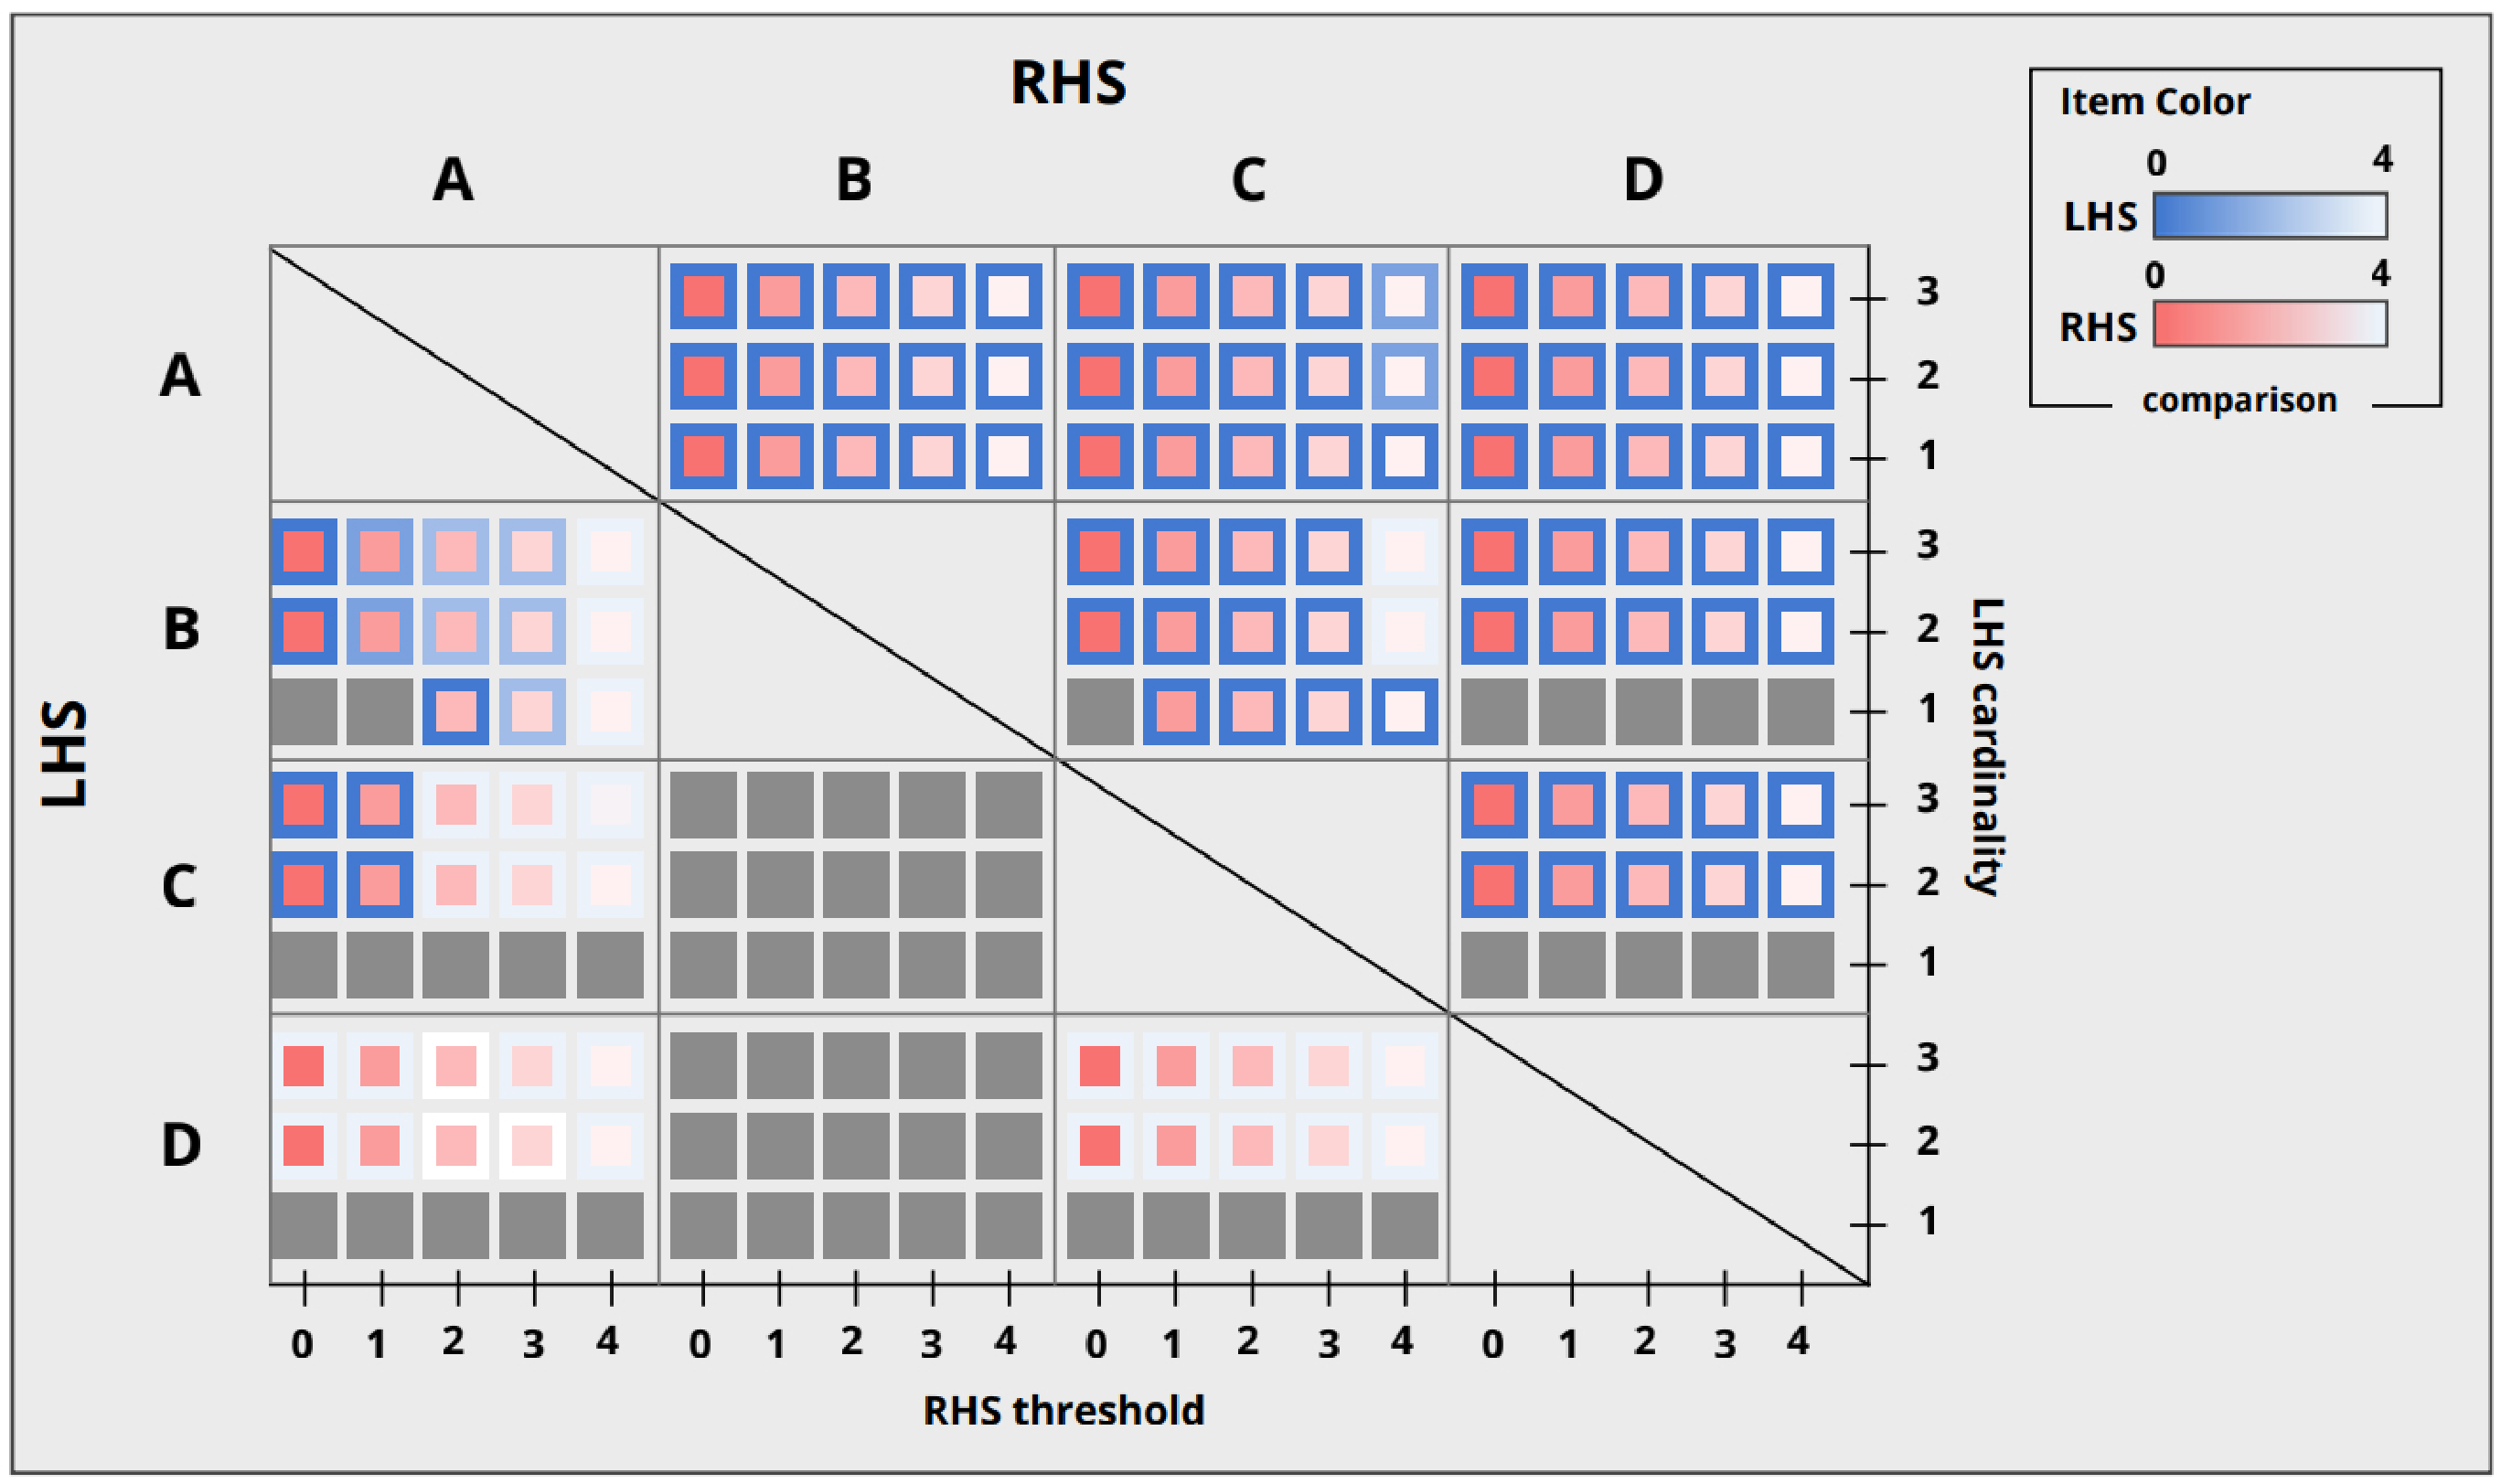
\includegraphics[width=\linewidth]{capitoli/figure/matrix_metaphore}
    \caption{Matrice colorata per una relazione con quattro attributi e soglie massime pari a 4.}
    \label{fig:colored_matrix}
\end{figure}
In questa sezione descriveremo una metafora per la visualizzazione di \acrshort{rfds} minimali \cite{mdvisualization}, scoperte dagli algoritmi di ricerca. La metafora che andremo a descrivere \`{e} una matrice colorata $n\times n$, come mostrato in Figura \ref{fig:colored_matrix}, dove $n$ rappresenta il numero di attributi. Questa prima metafora fornisce una panoramica sulle combinazioni di attributi su cui esiste una \acrshort{rfd} minimale, includendo la rappresentazione delle soglie di somiglianza corrispondenti basata su scale di gradienti di colore lineare. Come gi\`{a} accennato, le dimensioni della matrice rappresentano tutti gli attributi del dataset, utilizzando la stessa posizione per un dato attributo su entrambe le dimensioni. Le colonne di tale matrice, rappresentano i possibili attributi presenti sul lato destro, con le relative soglie associate. Le righe, invece, rappresentano le cardinalit\`{a} delle \acrshort{rfds} minimali includendo l'attributo di riga sul lato sinistro, con possibili soglie associate. Per esempio, consideriamo la sottomatrice $3\times5$ con le colonne associate all'attributo $A$ e le righe associate all'attributo $B$ nella Fig. \ref{fig:colored_matrix}. La riga in basso evidenzia se ci sono \acrshort{rfds} minimali con $B$ sul lato sinistro, la riga successiva evidenzia quelle che includono l'attributo $B$ con una cardinalit\`{a} del lato sinistra uguale a 2 (i.e., $BC$ o $BD$), ed infine, l'ultima riga evidenzia quelle che includono l'attributo $B$ con una cardinalit\`{a} del lato sinistro uguale a 3 (i.e., $BCD$). Le celle rappresentate in grigio indicano che non vi sono \acrshort{rfds} minimali con quelle caratteristiche, altrimenti sarebbero rappresentate con una sfumatura di rosso per lo sfondo ed il bordo con una sfumatura di blu. La sfumatura di rosso presente come sfondo delle celle rappresenta la soglia del lato destro, mentre la sfumatura di blu presente sul bordo delle celle rappresenta la soglia del lato sinistro, per cui colori pi\`{u} intensi rappresentano soglie pi\`{u} basse.\par
La matrice colorata, come descritta sopra, fornisce una panoramica delle correlazioni tra attributi mediante \acrlong{rfds}. Come esempio, il gruppo di colonne corrispondenti all'attributo $B$ nel lato destro mostrano che l'attributo \`{e} correlato solo all'attributo $A$, poich\'{e} le restanti sono tutte colorate di grigio. Allo stesso modo, il gruppo di colonne corrispondenti all'attributo $C$ sul lato destro rivelano che tale attributo ha pi\`{u} correlazioni con gli altri attributi, poich\'{e} ha poche celle colorate di grigio. Inoltre, guardando le ultime tre righe, si pu\`{o} notare che l'attributo $D$ appare nel lato sinistro di alcune \acrlong{rfds} solo in combinazione con altri attributi. Tali dipendenze hanno soglie alte sul lato sinistro (i bordi delle celle hanno un colore meno intenso) e consentono di ottenere \acrlong{rfds} minimali con soglie basse nel lato destro. Infine, la sotto-matrice corrispondente all'attributo di riga $B$ ed all'attributo di colonna $A$ rivela che esiste un'alta variabilit\`{a} delle soglie nelle \acrlong{rfds} aventi $B$ nel lato sinistro ed $A$ nel lato destro, poich\'{e} l'intensit\`{a} dei colori dei bordi diminuisce all'aumentare della soglia del lato destro.